% Energy landscape + annealed descent to a crystal (local minimum).
\begin{figure}[t]
\centering
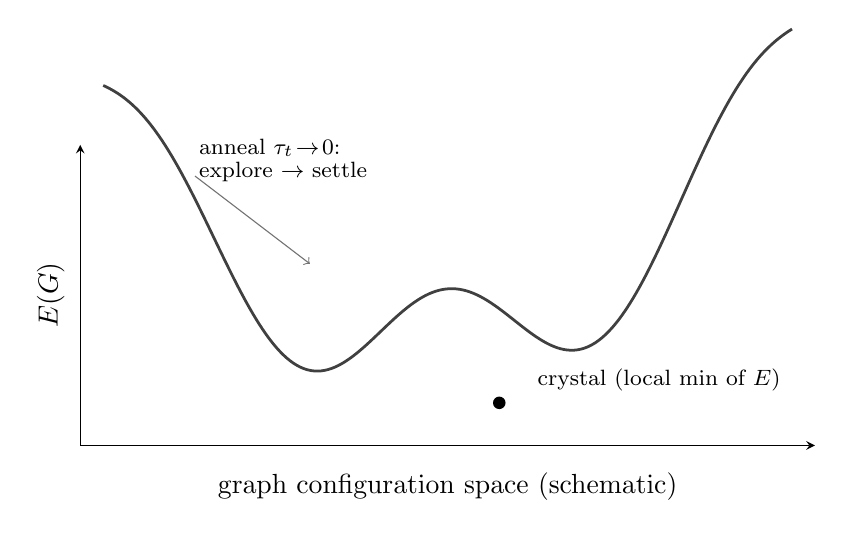
\begin{tikzpicture}
\begin{axis}[
  width=0.9\linewidth, height=5.4cm,
  xlabel={graph configuration space (schematic)},
  ylabel={$E(G)$},
  xmin=-3.2, xmax=3.2, ymin=-1.6, ymax=3.2,
  xtick=\empty, ytick=\empty,
  axis lines=left, every axis x label/.style={at={(axis description cs:0.5,-0.06)},anchor=north},
  clip=false,
]
% A bumpy energy curve with several wells.
\addplot[black!75, line width=1pt, samples=200, domain=-3:3]
  {0.45*x*x + 0.9*cos(deg(2.4*x)) + 0.15*x};
% Mark a local minimum near x = 0.45 (a "crystal").
\node[circle, fill=black, inner sep=1.6pt] (cryst) at (axis cs:0.45,-0.92) {};
\node[anchor=west, font=\footnotesize] at (axis cs:0.7,-0.55) {crystal (local min of $E$)};
% Annealing annotation.
\draw[->, black!55] (axis cs:-2.2,2.7) -- (axis cs:-1.2,1.3);
\node[anchor=west, font=\footnotesize, align=left] at (axis cs:-2.25,2.95)
  {anneal $\tau_t\!\to\!0$:\\[-1pt] explore $\to$ settle};
\end{axis}
\end{tikzpicture}
\caption{Crystallization as annealed descent. At high temperature the sampler
explores broadly; as $\tau_t\to 0$ it concentrates on a local minimum of the
energy $E$ within the gate-passing manifold --- a \emph{crystal}: a fixed point
where the projection is idempotent and no accepted move lowers $E$. As in
practical diffusion, the guarantee is local, not global.}
\label{fig:landscape}
\end{figure}
